Observability is the ability to check and visualize the state of the overall system. It is especially important with microservice architecture as complexity is increasing along with the decoupling of the services. There are also multiple data sources that need to be combined together to provide insight into component interactions. 

Figure \ref{fig:observability_system} shows the design of the observability system for this project. In a standard cloud-based application, all metrics are directly scraped by metric scrapers, which was implemented in a local setup. In a real system, some components are not deployed in the cloud (f.e agents) and therefore metrics need to be transported to the service which is deployed in the cloud - in this case, the backend service. Later those metrics are exposed to the metric collector.

\begin{figure}[H]
    \centering
    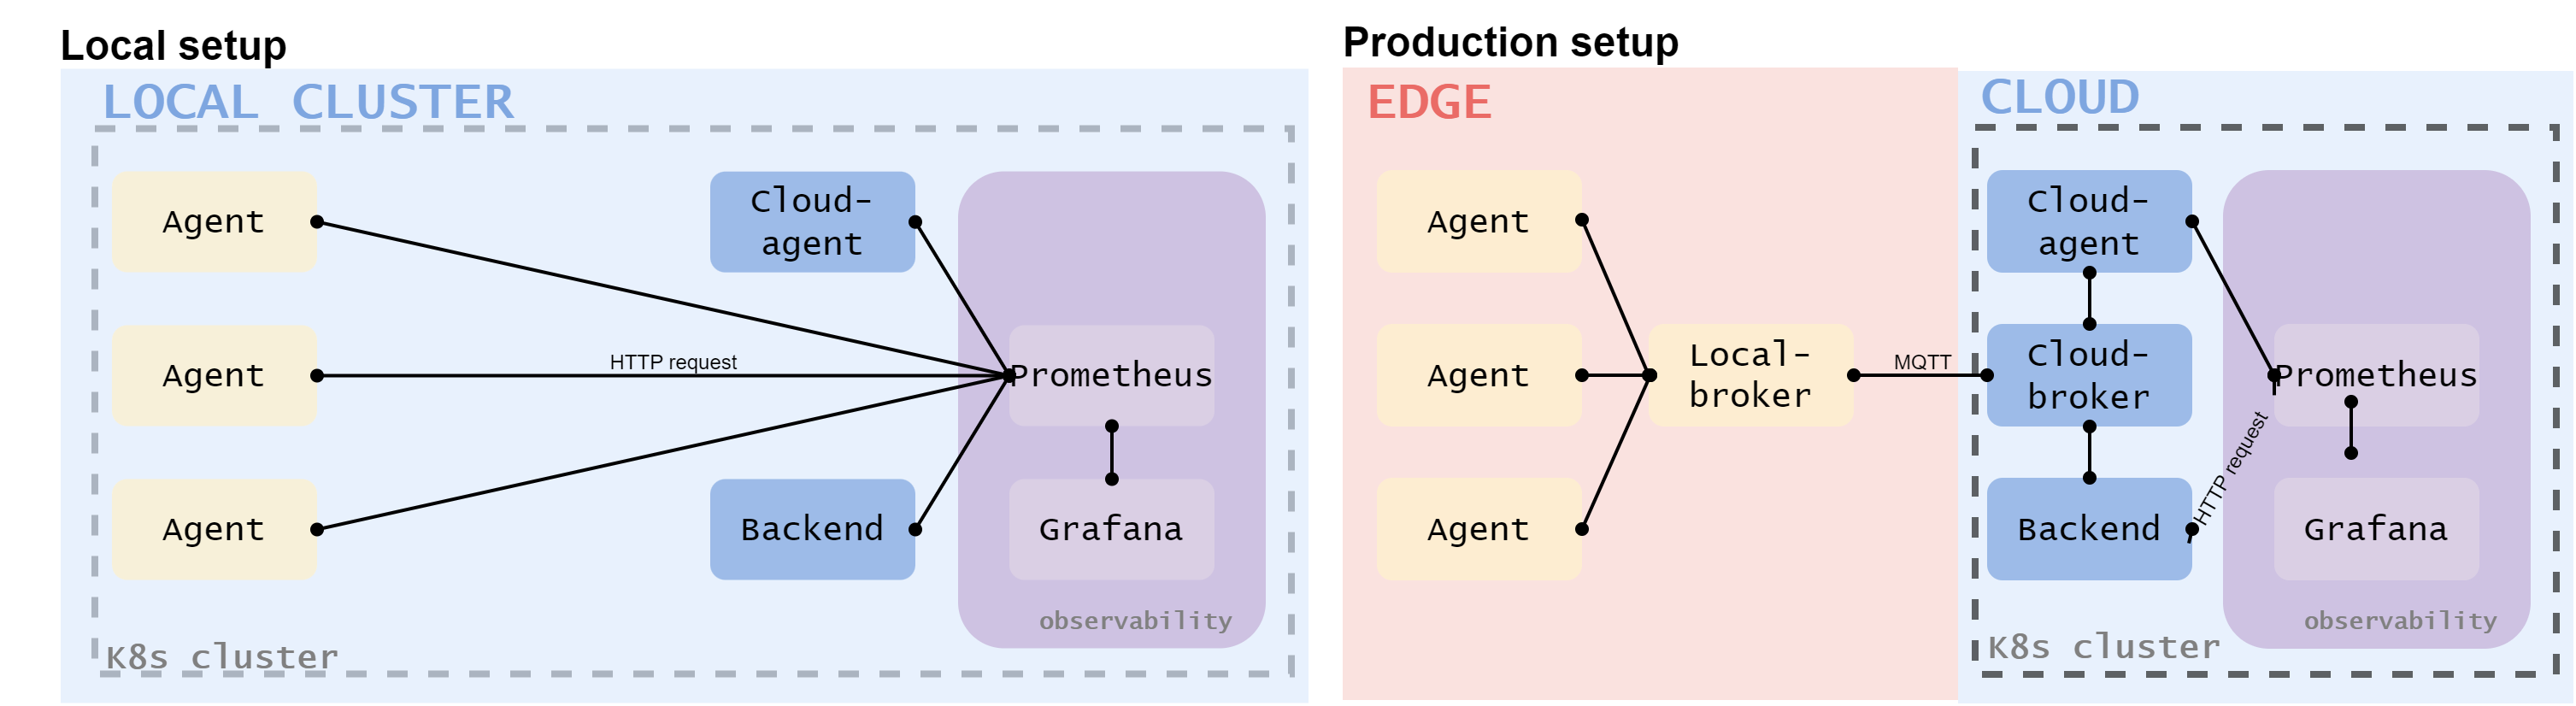
\includegraphics[width=\textwidth]{pictures/observability.png}
    \caption{Observability design}
    \label{fig:observability_system}
\end{figure}

Two open-source components are used in order to create an observability stack: Grafana and Prometheus. Prometheus is a monitoring solution that scrapes metrics from the HTTP endpoint, in the case of Kubernetes it scrapes metrics from pods whose metric monitor service is exposed. Prometheus later stores collected data in a time-series database and provide a way to query the data using the specific language (Prometheus Query Language) \cite{prometheus_docs}.

Grafana is meant as a visualization tool. It uses Prometheus queries to show data in form of charts, graphs, and other visualizations. In this project, multiple grafana dashboards were created to monitor the status of the system and the performance of the solution. An example can be seen in the figure \ref{fig:dashboard_grafana}.

\begin{figure}[H]
    \centering
    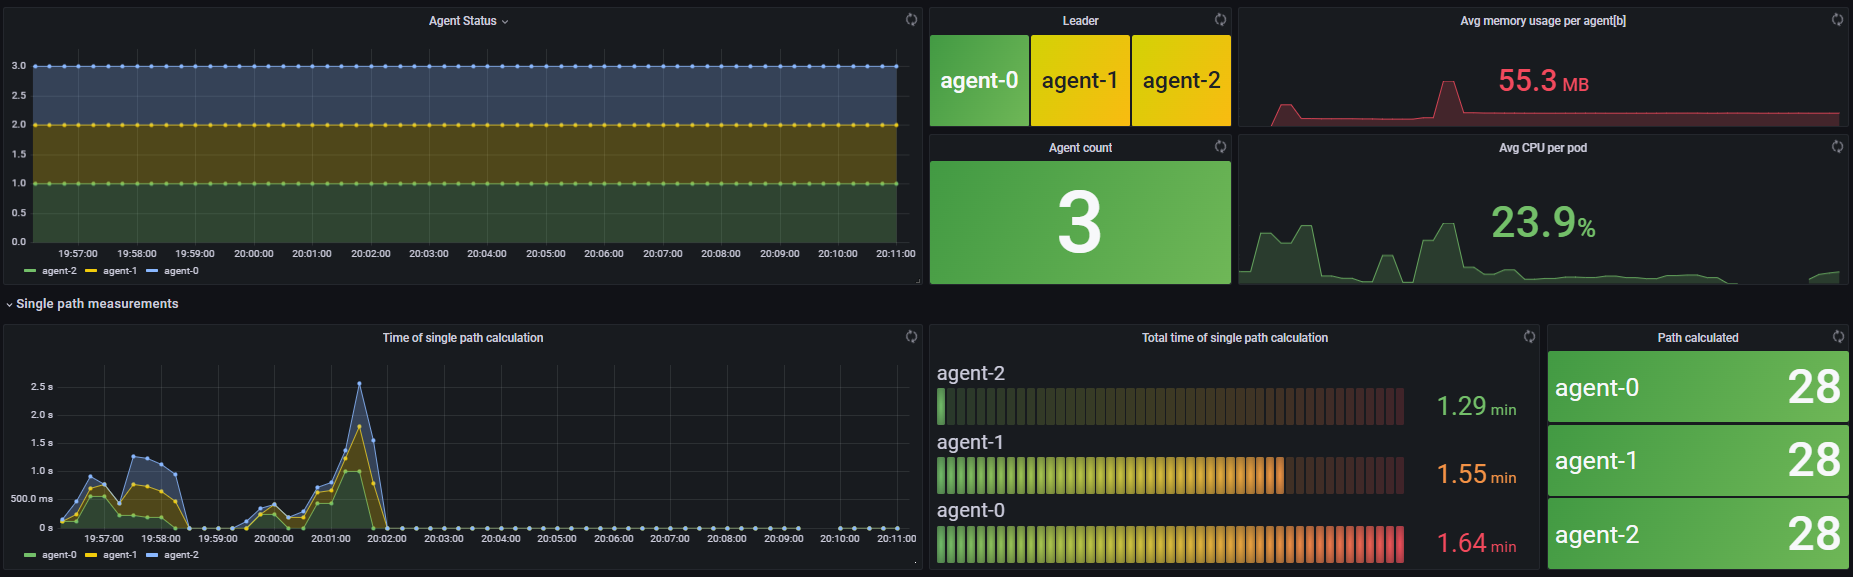
\includegraphics[width=\textwidth]{pictures/grafana.png}
    \caption{Dashboard in grafana}
    \label{fig:dashboard_grafana}
\end{figure}

The observability solution is capable of visualizing various aspects of the agents' performance, including their uptime, the current leader, the average memory and CPU utilization of the agents, the time taken for path calculation, and the number of paths found.
